\section{Deterministic finite automata}

\begin{definition}
    A \emph{finite deterministic automaton M} comprises five items:
    \begin{enumerate}
        \item $Q$, the state set (finite and not empty). 
        \item $\Sigma$, the input or terminal alphabet
        \item $\delta:(Q \times \Sigma) \rightarrow Q$, the transition function.
        \item $q_0 \in Q$, the initial state. 
        \item $F\subseteq Q$, the set of final states.
    \end{enumerate}
\end{definition}
Function $\delta$ specifies the moves: the meaning of $\delta(q,a)=r$ is that machine $M$ in the current state $q$ reads $a$ and moves to next state $r$. 
If $\delta(q,a)$ is undefined, the automaton stops, and we can assume it enters the error state. 

A special case is the empty string, for which we assume no change of state: 
\[\forall q \in Q:\delta(q,\varepsilon)=q\]
\begin{definition}
    The languages accepted by such automata are called \emph{finite-state recognizable}.
    
    Two automata are \emph{equivalent} if they accept the same language.
\end{definition}
Observing that for each input character the automaton executes one step, the total number of steps is exactly equal to the length of the input string. Therefore, such
machines are very efficient as they can recognize strings in real time by a single left-to-right scan.

\subsection*{Error state and total automata}
If the move is not defined in state $q$ when reading character $a$, we say that the automaton falls into the error state $q_{err}$. The error state is such that for 
any character the automaton remains in it, thus justifying its other name of sink or trap state. Obviously the error state is not final. The state-transition function 
can be made total by adding the error state and the transitions from/to it. 

Clearly any computation reaching the error state gets trapped in it and cannot reach a final state. As a consequence, the total automaton accepts the same language as 
the original one. It is customary to leave the error state implicit, neither drawing a node nor specifying the transitions for it.

\subsection*{Clean automata}
An automaton may contain useless parts not contributing to any accepting computation, which are best eliminated.
\begin{definition}
    A state $q$ is \emph{reachable} from state $p$ if a computation exists going from $p$ to $q$.

    A state is \emph{accessible} if it can be reached from the initial state. 

    A state is \emph{post-accessible} if a final state can be reached from it. 

    A state is called \emph{useful} if it is accessible and post-accessible. 

    An automaton is \emph{clean} if every state is useful.
\end{definition}
For every finite automaton there exists an equivalent clean automaton.

\subsection*{Minimal automata}
For every finite-state language, the deterministic finite recognizer minimal with respect to the number of states is unique.
\begin{definition}
    The states $p$ and $q$ are \emph{indistinguishable} if, and only if, for every string $x \in \Sigma^{*}$, either both states $\delta(p,x)$ and $\delta(q,x)$ are 
    final, or neither one is. 
    
    The complementary relation is termed \emph{distinguishability}.
\end{definition}
Two states $p$ and $q$ are indistinguishable if, starting from them and scanning the same arbitrarily chosen input string $x$, it never happens that a computation 
reaches a final state and the other does not. Notice that: 
\begin{enumerate}
    \item The sink state $q_{err}$ is distinguishable from every state $p$, since for any state there exists a string $x$ such that $\delta(p,x) \in F$, while for 
        every string $x$ it is $\delta(q_{err},x)=q_{err}$. 
    \item $p$ and $q$ are distinguishable if $p$ is final and $q$ is not, because $\delta(p,\varepsilon)\in F$ and $\delta(q,\varepsilon) \notin F$. 
    \item $p$ and $q$ are distinguishable if, for some character $a$, the next states $\delta(p,a)$ and $\delta(q,a)$ are distinguishable.
\end{enumerate}
In particular, $p$ is distinguishable from $q$ if the set of labels attached to the outgoing arrows from $p$ and the similar set from $q$ are different. 

Indistinguishability as a relation is symmetric, reflexive, and transitive. 

\subsection*{Construction of minimal automaton}
The minimal automaton $M^{'}$, equivalent to the given $M$, has for states the equivalence classes of the indistinguishability relation. From this it is a 
straightforward test to check whether two given machines are equivalent. First minimize both machines; then compare their state-transition graphs to see if 
they are identical. In practical use, obvious economy reasons make the minimal machine a prefer-able  choice. But the saving is often negligible for  
the cases of concern in compiler design. What is more, in certain situations state minimization of the recognizer should be avoided. The uniqueness property 
of the minimal automaton does not hold for the nondeterministic machines. 

\subsection*{From automaton to grammars}
The grammar $G$ has as non-terminal set the states $Q$ of the automaton, and the axiom is the initial state. For each move $q \rightarrow^{a} r$ the grammar 
has the rule $q \rightarrow ar$. If state $q$ is final, it has also the terminal rule $q \rightarrow \varepsilon$. It is evident that there exists a bijective 
correspondence between the computations of the automaton and the derivations of the grammar. 
\begin{example}
    The correspondence between an automaton and a grammar is shown below. 
    \begin{figure}[H]
        \centering
        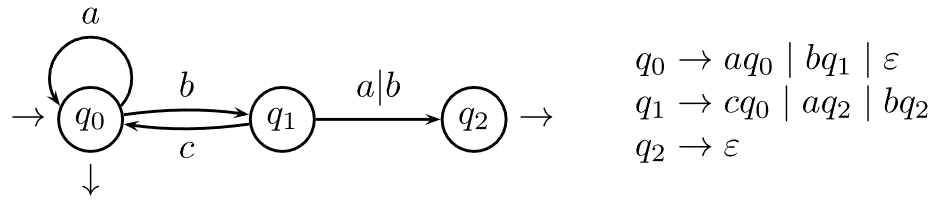
\includegraphics[width=0.9\linewidth]{images/autgram.png}
    \end{figure}
\end{example}
The conversion from automaton to grammar has been straightforward, but to make the reverse transformation from grammar to automaton, we need to 
modify the machine definition by permitting nondeterministic behavior.